\documentclass[1p]{elsarticle_modified}
%\bibliographystyle{elsarticle-num}

%\usepackage[colorlinks]{hyperref}
%\usepackage{abbrmath_seonhwa} %\Abb, \Ascr, \Acal ,\Abf, \Afrak
\usepackage{amsfonts}
\usepackage{amssymb}
\usepackage{amsmath}
\usepackage{amsthm}
\usepackage{scalefnt}
\usepackage{amsbsy}
\usepackage{kotex}
\usepackage{caption}
\usepackage{subfig}
\usepackage{color}
\usepackage{graphicx}
\usepackage{xcolor} %% white, black, red, green, blue, cyan, magenta, yellow
\usepackage{float}
\usepackage{setspace}
\usepackage{hyperref}

\usepackage{tikz}
\usetikzlibrary{arrows}

\usepackage{multirow}
\usepackage{array} % fixed length table
\usepackage{hhline}

%%%%%%%%%%%%%%%%%%%%%
\makeatletter
\renewcommand*\env@matrix[1][\arraystretch]{%
	\edef\arraystretch{#1}%
	\hskip -\arraycolsep
	\let\@ifnextchar\new@ifnextchar
	\array{*\c@MaxMatrixCols c}}
\makeatother %https://tex.stackexchange.com/questions/14071/how-can-i-increase-the-line-spacing-in-a-matrix
%%%%%%%%%%%%%%%

\usepackage[normalem]{ulem}

\newcommand{\msout}[1]{\ifmmode\text{\sout{\ensuremath{#1}}}\else\sout{#1}\fi}
%SOURCE: \msout is \stkout macro in https://tex.stackexchange.com/questions/20609/strikeout-in-math-mode

\newcommand{\cancel}[1]{
	\ifmmode
	{\color{red}\msout{#1}}
	\else
	{\color{red}\sout{#1}}
	\fi
}

\newcommand{\add}[1]{
	{\color{blue}\uwave{#1}}
}

\newcommand{\replace}[2]{
	\ifmmode
	{\color{red}\msout{#1}}{\color{blue}\uwave{#2}}
	\else
	{\color{red}\sout{#1}}{\color{blue}\uwave{#2}}
	\fi
}

\newcommand{\Sol}{\mathcal{S}} %segment
\newcommand{\D}{D} %diagram
\newcommand{\A}{\mathcal{A}} %arc


%%%%%%%%%%%%%%%%%%%%%%%%%%%%%5 test

\def\sl{\operatorname{\textup{SL}}(2,\Cbb)}
\def\psl{\operatorname{\textup{PSL}}(2,\Cbb)}
\def\quan{\mkern 1mu \triangleright \mkern 1mu}

\theoremstyle{definition}
\newtheorem{thm}{Theorem}[section]
\newtheorem{prop}[thm]{Proposition}
\newtheorem{lem}[thm]{Lemma}
\newtheorem{ques}[thm]{Question}
\newtheorem{cor}[thm]{Corollary}
\newtheorem{defn}[thm]{Definition}
\newtheorem{exam}[thm]{Example}
\newtheorem{rmk}[thm]{Remark}
\newtheorem{alg}[thm]{Algorithm}

\newcommand{\I}{\sqrt{-1}}
\begin{document}

%\begin{frontmatter}
%
%\title{Boundary parabolic representations of knots up to 8 crossings}
%
%%% Group authors per affiliation:
%\author{Yunhi Cho} 
%\address{Department of Mathematics, University of Seoul, Seoul, Korea}
%\ead{yhcho@uos.ac.kr}
%
%
%\author{Seonhwa Kim} %\fnref{s_kim}}
%\address{Center for Geometry and Physics, Institute for Basic Science, Pohang, 37673, Korea}
%\ead{ryeona17@ibs.re.kr}
%
%\author{Hyuk Kim}
%\address{Department of Mathematical Sciences, Seoul National University, Seoul 08826, Korea}
%\ead{hyukkim@snu.ac.kr}
%
%\author{Seokbeom Yoon}
%\address{Department of Mathematical Sciences, Seoul National University, Seoul, 08826,  Korea}
%\ead{sbyoon15@snu.ac.kr}
%
%\begin{abstract}
%We find all boundary parabolic representation of knots up to 8 crossings.
%
%\end{abstract}
%\begin{keyword}
%    \MSC[2010] 57M25 
%\end{keyword}
%
%\end{frontmatter}

%\linenumbers
%\tableofcontents
%
\newcommand\colored[1]{\textcolor{white}{\rule[-0.35ex]{0.8em}{1.4ex}}\kern-0.8em\color{red} #1}%
%\newcommand\colored[1]{\textcolor{white}{ #1}\kern-2.17ex	\textcolor{white}{ #1}\kern-1.81ex	\textcolor{white}{ #1}\kern-2.15ex\color{red}#1	}

{\Large $\underline{10_{82}~(K10a_{83})}$}

\setlength{\tabcolsep}{10pt}
\renewcommand{\arraystretch}{1.6}
\vspace{1cm}\begin{tabular}{m{100pt}>{\centering\arraybackslash}m{274pt}}
\multirow{5}{120pt}{
	\centering
	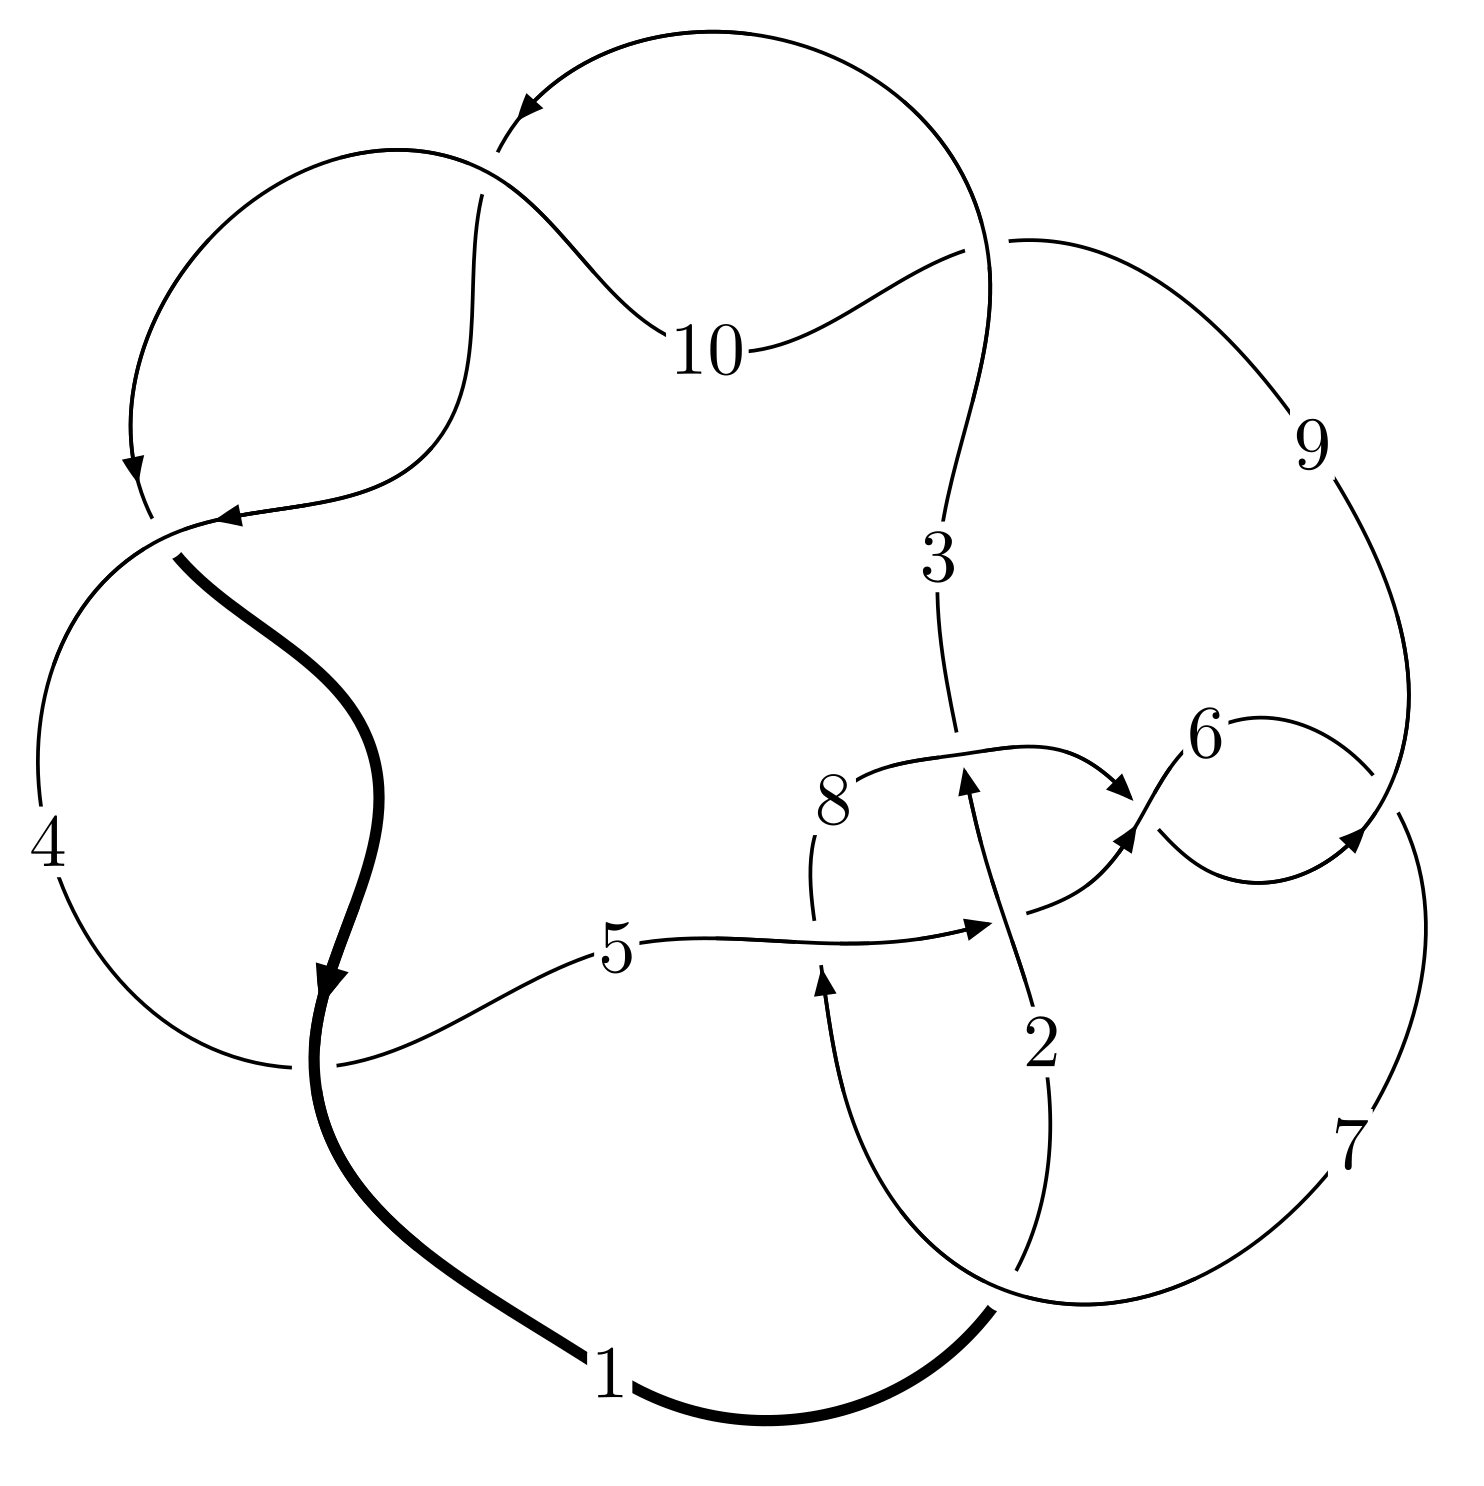
\includegraphics[width=112pt]{../../../GIT/diagram.site/Diagrams/png/166_10_82.png}\\
\ \ \ A knot diagram\footnotemark}&
\allowdisplaybreaks
\textbf{Linearized knot diagam} \\
\cline{2-2}
 &
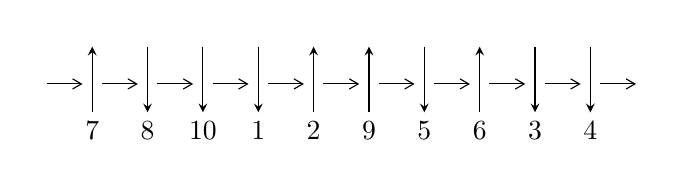
\begin{tikzpicture}[x=20pt, y=17pt]
	% nodes
	\node (C0) at (0, 0) {};
	\node (C1) at (1, 0) {};
	\node (C1U) at (1, +1) {};
	\node (C1D) at (1, -1) {7};

	\node (C2) at (2, 0) {};
	\node (C2U) at (2, +1) {};
	\node (C2D) at (2, -1) {8};

	\node (C3) at (3, 0) {};
	\node (C3U) at (3, +1) {};
	\node (C3D) at (3, -1) {10};

	\node (C4) at (4, 0) {};
	\node (C4U) at (4, +1) {};
	\node (C4D) at (4, -1) {1};

	\node (C5) at (5, 0) {};
	\node (C5U) at (5, +1) {};
	\node (C5D) at (5, -1) {2};

	\node (C6) at (6, 0) {};
	\node (C6U) at (6, +1) {};
	\node (C6D) at (6, -1) {9};

	\node (C7) at (7, 0) {};
	\node (C7U) at (7, +1) {};
	\node (C7D) at (7, -1) {5};

	\node (C8) at (8, 0) {};
	\node (C8U) at (8, +1) {};
	\node (C8D) at (8, -1) {6};

	\node (C9) at (9, 0) {};
	\node (C9U) at (9, +1) {};
	\node (C9D) at (9, -1) {3};

	\node (C10) at (10, 0) {};
	\node (C10U) at (10, +1) {};
	\node (C10D) at (10, -1) {4};
	\node (C11) at (11, 0) {};

	% arrows
	\draw[->,>={angle 60}]
	(C0) edge (C1) (C1) edge (C2) (C2) edge (C3) (C3) edge (C4) (C4) edge (C5) (C5) edge (C6) (C6) edge (C7) (C7) edge (C8) (C8) edge (C9) (C9) edge (C10) (C10) edge (C11) ;	\draw[->,>=stealth]
	(C1D) edge (C1U) (C2U) edge (C2D) (C3U) edge (C3D) (C4U) edge (C4D) (C5D) edge (C5U) (C6D) edge (C6U) (C7U) edge (C7D) (C8D) edge (C8U) (C9U) edge (C9D) (C10U) edge (C10D) ;
	\end{tikzpicture} \\
\hhline{~~} \\& 
\textbf{Solving Sequence} \\ \cline{2-2} 
 &
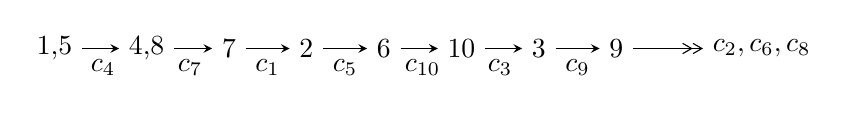
\begin{tikzpicture}[x=28pt, y=7pt]
	% node
	\node (A0) at (-1/8, 0) {1,5};
	\node (A1) at (17/16, 0) {4,8};
	\node (A2) at (17/8, 0) {7};
	\node (A3) at (25/8, 0) {2};
	\node (A4) at (33/8, 0) {6};
	\node (A5) at (41/8, 0) {10};
	\node (A6) at (49/8, 0) {3};
	\node (A7) at (57/8, 0) {9};
	\node (C1) at (1/2, -1) {$c_{4}$};
	\node (C2) at (13/8, -1) {$c_{7}$};
	\node (C3) at (21/8, -1) {$c_{1}$};
	\node (C4) at (29/8, -1) {$c_{5}$};
	\node (C5) at (37/8, -1) {$c_{10}$};
	\node (C6) at (45/8, -1) {$c_{3}$};
	\node (C7) at (53/8, -1) {$c_{9}$};
	\node (A8) at (9, 0) {$c_{2},c_{6},c_{8}$};

	% edge
	\draw[->,>=stealth]	
	(A0) edge (A1) (A1) edge (A2) (A2) edge (A3) (A3) edge (A4) (A4) edge (A5) (A5) edge (A6) (A6) edge (A7) ;
	\draw[->>,>={angle 60}]	
	(A7) edge (A8);
\end{tikzpicture} \\ 

\end{tabular} \\

\footnotetext{
The image of knot diagram is generated by the software ``\textbf{Draw programme}" developed by Andrew Bartholomew(\url{http://www.layer8.co.uk/maths/draw/index.htm\#Running-draw}), where we modified some parts for our purpose(\url{https://github.com/CATsTAILs/LinksPainter}).
}\phantom \\ \newline 
\centering \textbf{Ideals for irreducible components\footnotemark of $X_{\text{par}}$} 
 
\begin{align*}
I^u_{1}&=\langle 
1790814371 u^{31}+3053908485 u^{30}+\cdots+15215838414 b+1796669401,\\
\phantom{I^u_{1}}&\phantom{= \langle  }9786061617 u^{31}+13386015963 u^{30}+\cdots+5071946138 a+29865915991,\;u^{32}+2 u^{31}+\cdots- u+1\rangle \\
I^u_{2}&=\langle 
b,\;a+1,\;u+1\rangle \\
\\
\end{align*}
\raggedright * 2 irreducible components of $\dim_{\mathbb{C}}=0$, with total 33 representations.\\
\footnotetext{All coefficients of polynomials are rational numbers. But the coefficients are sometimes approximated in decimal forms when there is not enough margin.}
\newpage
\renewcommand{\arraystretch}{1}
\centering \section*{I. $I^u_{1}= \langle 1.79\times10^{9} u^{31}+3.05\times10^{9} u^{30}+\cdots+1.52\times10^{10} b+1.80\times10^{9},\;9.79\times10^{9} u^{31}+1.34\times10^{10} u^{30}+\cdots+5.07\times10^{9} a+2.99\times10^{10},\;u^{32}+2 u^{31}+\cdots- u+1 \rangle$}
\flushleft \textbf{(i) Arc colorings}\\
\begin{tabular}{m{7pt} m{180pt} m{7pt} m{180pt} }
\flushright $a_{1}=$&$\begin{pmatrix}0\\u\end{pmatrix}$ \\
\flushright $a_{5}=$&$\begin{pmatrix}1\\0\end{pmatrix}$ \\
\flushright $a_{4}=$&$\begin{pmatrix}1\\- u^2\end{pmatrix}$ \\
\flushright $a_{8}=$&$\begin{pmatrix}-1.92945 u^{31}-2.63923 u^{30}+\cdots+9.12108 u-5.88845\\-0.117694 u^{31}-0.200706 u^{30}+\cdots+2.07712 u-0.118079\end{pmatrix}$ \\
\flushright $a_{7}=$&$\begin{pmatrix}-2.04714 u^{31}-2.83993 u^{30}+\cdots+11.1982 u-6.00653\\-0.117694 u^{31}-0.200706 u^{30}+\cdots+2.07712 u-0.118079\end{pmatrix}$ \\
\flushright $a_{2}=$&$\begin{pmatrix}-2.22835 u^{31}-3.03012 u^{30}+\cdots+0.715268 u+0.285838\\-0.998715 u^{31}-0.999372 u^{30}+\cdots+1.28281 u-0.999382\end{pmatrix}$ \\
\flushright $a_{6}=$&$\begin{pmatrix}2.22354 u^{31}+3.04014 u^{30}+\cdots-10.0154 u+6.22362\\- u^5+3 u^3- u\end{pmatrix}$ \\
\flushright $a_{10}=$&$\begin{pmatrix}u\\- u^3+u\end{pmatrix}$ \\
\flushright $a_{3}=$&$\begin{pmatrix}- u^2+1\\u^4-2 u^2\end{pmatrix}$ \\
\flushright $a_{9}=$&$\begin{pmatrix}- u^3+2 u\\u^5-3 u^3+u\end{pmatrix}$\\&\end{tabular}
\flushleft \textbf{(ii) Obstruction class $= -1$}\\~\\
\flushleft \textbf{(iii) Cusp Shapes $= \frac{18210579048}{2535973069} u^{31}+\frac{32359838926}{2535973069} u^{30}+\cdots-\frac{94883406442}{2535973069} u+\frac{41946667180}{2535973069}$}\\~\\
\newpage\renewcommand{\arraystretch}{1}
\flushleft \textbf{(iv) u-Polynomials at the component}\newline \\
\begin{tabular}{m{50pt}|m{274pt}}
Crossings & \hspace{64pt}u-Polynomials at each crossing \\
\hline $$\begin{aligned}c_{1}\end{aligned}$$&$\begin{aligned}
&u^{32}+2 u^{31}+\cdots+12 u+8
\end{aligned}$\\
\hline $$\begin{aligned}c_{2}\end{aligned}$$&$\begin{aligned}
&u^{32}+11 u^{30}+\cdots+13 u-1
\end{aligned}$\\
\hline $$\begin{aligned}c_{3},c_{4},c_{9}\\c_{10}\end{aligned}$$&$\begin{aligned}
&u^{32}+2 u^{31}+\cdots- u+1
\end{aligned}$\\
\hline $$\begin{aligned}c_{5}\end{aligned}$$&$\begin{aligned}
&u^{32}-2 u^{31}+\cdots+u-1
\end{aligned}$\\
\hline $$\begin{aligned}c_{6},c_{8}\end{aligned}$$&$\begin{aligned}
&u^{32}+2 u^{31}+\cdots-13 u-1
\end{aligned}$\\
\hline $$\begin{aligned}c_{7}\end{aligned}$$&$\begin{aligned}
&u^{32}-5 u^{31}+\cdots-6 u+2
\end{aligned}$\\
\hline
\end{tabular}\\~\\
\newpage\renewcommand{\arraystretch}{1}
\flushleft \textbf{(v) Riley Polynomials at the component}\newline \\
\begin{tabular}{m{50pt}|m{274pt}}
Crossings & \hspace{64pt}Riley Polynomials at each crossing \\
\hline $$\begin{aligned}c_{1}\end{aligned}$$&$\begin{aligned}
&y^{32}+30 y^{31}+\cdots+240 y+64
\end{aligned}$\\
\hline $$\begin{aligned}c_{2}\end{aligned}$$&$\begin{aligned}
&y^{32}+22 y^{31}+\cdots-121 y+1
\end{aligned}$\\
\hline $$\begin{aligned}c_{3},c_{4},c_{9}\\c_{10}\end{aligned}$$&$\begin{aligned}
&y^{32}-38 y^{31}+\cdots-5 y+1
\end{aligned}$\\
\hline $$\begin{aligned}c_{5}\end{aligned}$$&$\begin{aligned}
&y^{32}-6 y^{31}+\cdots-5 y+1
\end{aligned}$\\
\hline $$\begin{aligned}c_{6},c_{8}\end{aligned}$$&$\begin{aligned}
&y^{32}-18 y^{31}+\cdots-81 y+1
\end{aligned}$\\
\hline $$\begin{aligned}c_{7}\end{aligned}$$&$\begin{aligned}
&y^{32}-9 y^{31}+\cdots-32 y+4
\end{aligned}$\\
\hline
\end{tabular}\\~\\
\newpage\flushleft \textbf{(vi) Complex Volumes and Cusp Shapes}
$$\begin{array}{c|c|c}  
\text{Solutions to }I^u_{1}& \I (\text{vol} + \sqrt{-1}CS) & \text{Cusp shape}\\
 \hline 
\begin{aligned}
u &= \phantom{-}0.820983 + 0.567595 I \\
a &= -1.27469 + 0.62091 I \\
b &= \phantom{-}1.088800 + 0.850114 I\end{aligned}
 & \phantom{-}0.60537 - 9.61260 I & -2.87987 + 8.20248 I \\ \hline\begin{aligned}
u &= \phantom{-}0.820983 - 0.567595 I \\
a &= -1.27469 - 0.62091 I \\
b &= \phantom{-}1.088800 - 0.850114 I\end{aligned}
 & \phantom{-}0.60537 + 9.61260 I & -2.87987 - 8.20248 I \\ \hline\begin{aligned}
u &= \phantom{-}0.795955 + 0.349102 I \\
a &= \phantom{-}1.45784 - 0.39446 I \\
b &= -1.136450 - 0.835713 I\end{aligned}
 & -2.75563 - 4.13382 I & -6.93448 + 6.73749 I \\ \hline\begin{aligned}
u &= \phantom{-}0.795955 - 0.349102 I \\
a &= \phantom{-}1.45784 + 0.39446 I \\
b &= -1.136450 + 0.835713 I\end{aligned}
 & -2.75563 + 4.13382 I & -6.93448 - 6.73749 I \\ \hline\begin{aligned}
u &= -0.643643 + 0.579820 I \\
a &= \phantom{-}0.109445 + 0.730653 I \\
b &= -0.758624 + 0.110290 I\end{aligned}
 & -1.27204 + 1.92248 I & -7.80216 - 5.91516 I \\ \hline\begin{aligned}
u &= -0.643643 - 0.579820 I \\
a &= \phantom{-}0.109445 - 0.730653 I \\
b &= -0.758624 - 0.110290 I\end{aligned}
 & -1.27204 - 1.92248 I & -7.80216 + 5.91516 I \\ \hline\begin{aligned}
u &= -1.076160 + 0.444148 I \\
a &= -0.311615 - 0.602654 I \\
b &= \phantom{-}0.691368 + 0.318391 I\end{aligned}
 & -0.800175 - 0.941991 I & -6.40540 + 5.25085 I \\ \hline\begin{aligned}
u &= -1.076160 - 0.444148 I \\
a &= -0.311615 + 0.602654 I \\
b &= \phantom{-}0.691368 - 0.318391 I\end{aligned}
 & -0.800175 + 0.941991 I & -6.40540 - 5.25085 I \\ \hline\begin{aligned}
u &= -0.788048\phantom{ +0.000000I} \\
a &= -0.997928\phantom{ +0.000000I} \\
b &= \phantom{-}0.333761\phantom{ +0.000000I}\end{aligned}
 & -1.36694\phantom{ +0.000000I} & -7.37900\phantom{ +0.000000I} \\ \hline\begin{aligned}
u &= \phantom{-}0.102445 + 0.771273 I \\
a &= \phantom{-}0.249085 - 0.151496 I \\
b &= \phantom{-}0.853465 - 0.688304 I\end{aligned}
 & \phantom{-}2.78249 + 5.16401 I & \phantom{-}0.17525 - 5.43243 I\\
 \hline 
 \end{array}$$\newpage$$\begin{array}{c|c|c}  
\text{Solutions to }I^u_{1}& \I (\text{vol} + \sqrt{-1}CS) & \text{Cusp shape}\\
 \hline 
\begin{aligned}
u &= \phantom{-}0.102445 - 0.771273 I \\
a &= \phantom{-}0.249085 + 0.151496 I \\
b &= \phantom{-}0.853465 + 0.688304 I\end{aligned}
 & \phantom{-}2.78249 - 5.16401 I & \phantom{-}0.17525 + 5.43243 I \\ \hline\begin{aligned}
u &= \phantom{-}0.560858 + 0.310184 I \\
a &= -0.155519 + 0.637386 I \\
b &= \phantom{-}0.671965 - 1.149150 I\end{aligned}
 & \phantom{-}1.86601 - 2.61443 I & \phantom{-}0.82365 + 8.13996 I \\ \hline\begin{aligned}
u &= \phantom{-}0.560858 - 0.310184 I \\
a &= -0.155519 - 0.637386 I \\
b &= \phantom{-}0.671965 + 1.149150 I\end{aligned}
 & \phantom{-}1.86601 + 2.61443 I & \phantom{-}0.82365 - 8.13996 I \\ \hline\begin{aligned}
u &= -0.598750 + 0.114970 I \\
a &= \phantom{-}0.25826 - 3.79474 I \\
b &= -0.135421 - 0.360183 I\end{aligned}
 & \phantom{-}0.576409 + 0.313871 I & \phantom{-}8.1378 + 17.1065 I \\ \hline\begin{aligned}
u &= -0.598750 - 0.114970 I \\
a &= \phantom{-}0.25826 + 3.79474 I \\
b &= -0.135421 + 0.360183 I\end{aligned}
 & \phantom{-}0.576409 - 0.313871 I & \phantom{-}8.1378 - 17.1065 I \\ \hline\begin{aligned}
u &= -0.086458 + 0.449548 I \\
a &= -0.783456 + 0.459529 I \\
b &= -0.610958 + 0.536174 I\end{aligned}
 & -0.227616 + 1.394370 I & -2.60146 - 4.04487 I \\ \hline\begin{aligned}
u &= -0.086458 - 0.449548 I \\
a &= -0.783456 - 0.459529 I \\
b &= -0.610958 - 0.536174 I\end{aligned}
 & -0.227616 - 1.394370 I & -2.60146 + 4.04487 I \\ \hline\begin{aligned}
u &= -1.55208\phantom{ +0.000000I} \\
a &= -2.62954\phantom{ +0.000000I} \\
b &= \phantom{-}1.76871\phantom{ +0.000000I}\end{aligned}
 & -3.73390\phantom{ +0.000000I} & \phantom{-0.000000 } 0 \\ \hline\begin{aligned}
u &= -1.57850 + 0.06009 I \\
a &= -0.52697 - 1.39477 I \\
b &= \phantom{-}0.56830 + 1.70360 I\end{aligned}
 & -5.46664 + 3.81790 I & \phantom{-0.000000 } 0 \\ \hline\begin{aligned}
u &= -1.57850 - 0.06009 I \\
a &= -0.52697 + 1.39477 I \\
b &= \phantom{-}0.56830 - 1.70360 I\end{aligned}
 & -5.46664 - 3.81790 I & \phantom{-0.000000 } 0\\
 \hline 
 \end{array}$$\newpage$$\begin{array}{c|c|c}  
\text{Solutions to }I^u_{1}& \I (\text{vol} + \sqrt{-1}CS) & \text{Cusp shape}\\
 \hline 
\begin{aligned}
u &= \phantom{-}1.60015 + 0.02565 I \\
a &= \phantom{-}0.830347 + 1.077280 I \\
b &= -0.363802 + 0.595725 I\end{aligned}
 & -7.09081 - 0.79638 I & \phantom{-0.000000 } 0 \\ \hline\begin{aligned}
u &= \phantom{-}1.60015 - 0.02565 I \\
a &= \phantom{-}0.830347 - 1.077280 I \\
b &= -0.363802 - 0.595725 I\end{aligned}
 & -7.09081 + 0.79638 I & \phantom{-0.000000 } 0 \\ \hline\begin{aligned}
u &= \phantom{-}0.269938 + 0.288721 I \\
a &= -2.52869 + 1.49962 I \\
b &= \phantom{-}0.887931 + 0.459497 I\end{aligned}
 & \phantom{-}2.64104 + 0.25879 I & \phantom{-}3.85203 + 2.96045 I \\ \hline\begin{aligned}
u &= \phantom{-}0.269938 - 0.288721 I \\
a &= -2.52869 - 1.49962 I \\
b &= \phantom{-}0.887931 - 0.459497 I\end{aligned}
 & \phantom{-}2.64104 - 0.25879 I & \phantom{-}3.85203 - 2.96045 I \\ \hline\begin{aligned}
u &= \phantom{-}1.61612 + 0.17777 I \\
a &= \phantom{-}1.092350 - 0.316288 I \\
b &= -0.985940 - 0.438836 I\end{aligned}
 & -8.99388 - 4.78654 I & \phantom{-0.000000 } 0 \\ \hline\begin{aligned}
u &= \phantom{-}1.61612 - 0.17777 I \\
a &= \phantom{-}1.092350 + 0.316288 I \\
b &= -0.985940 + 0.438836 I\end{aligned}
 & -8.99388 + 4.78654 I & \phantom{-0.000000 } 0 \\ \hline\begin{aligned}
u &= -1.63927 + 0.09770 I \\
a &= \phantom{-}2.05679 - 0.27434 I \\
b &= -1.51522 + 0.94459 I\end{aligned}
 & -11.15790 + 5.83644 I & \phantom{-0.000000 } 0 \\ \hline\begin{aligned}
u &= -1.63927 - 0.09770 I \\
a &= \phantom{-}2.05679 + 0.27434 I \\
b &= -1.51522 - 0.94459 I\end{aligned}
 & -11.15790 - 5.83644 I & \phantom{-0.000000 } 0 \\ \hline\begin{aligned}
u &= -1.65031 + 0.16673 I \\
a &= -1.89221 + 0.02470 I \\
b &= \phantom{-}1.30041 - 0.93941 I\end{aligned}
 & -7.8166 + 12.4315 I & \phantom{-0.000000 } 0 \\ \hline\begin{aligned}
u &= -1.65031 - 0.16673 I \\
a &= -1.89221 - 0.02470 I \\
b &= \phantom{-}1.30041 + 0.93941 I\end{aligned}
 & -7.8166 - 12.4315 I & \phantom{-0.000000 } 0\\
 \hline 
 \end{array}$$\newpage$$\begin{array}{c|c|c}  
\text{Solutions to }I^u_{1}& \I (\text{vol} + \sqrt{-1}CS) & \text{Cusp shape}\\
 \hline 
\begin{aligned}
u &= \phantom{-}1.67671 + 0.06666 I \\
a &= -1.267240 + 0.207888 I \\
b &= \phantom{-}0.892941 + 0.200725 I\end{aligned}
 & -10.51010 - 0.53898 I & \phantom{-0.000000 } 0 \\ \hline\begin{aligned}
u &= \phantom{-}1.67671 - 0.06666 I \\
a &= -1.267240 - 0.207888 I \\
b &= \phantom{-}0.892941 - 0.200725 I\end{aligned}
 & -10.51010 + 0.53898 I & \phantom{-0.000000 } 0\\
 \hline 
 \end{array}$$\newpage\newpage\renewcommand{\arraystretch}{1}
\centering \section*{II. $I^u_{2}= \langle b,\;a+1,\;u+1 \rangle$}
\flushleft \textbf{(i) Arc colorings}\\
\begin{tabular}{m{7pt} m{180pt} m{7pt} m{180pt} }
\flushright $a_{1}=$&$\begin{pmatrix}0\\-1\end{pmatrix}$ \\
\flushright $a_{5}=$&$\begin{pmatrix}1\\0\end{pmatrix}$ \\
\flushright $a_{4}=$&$\begin{pmatrix}1\\-1\end{pmatrix}$ \\
\flushright $a_{8}=$&$\begin{pmatrix}-1\\0\end{pmatrix}$ \\
\flushright $a_{7}=$&$\begin{pmatrix}-1\\0\end{pmatrix}$ \\
\flushright $a_{2}=$&$\begin{pmatrix}-1\\-1\end{pmatrix}$ \\
\flushright $a_{6}=$&$\begin{pmatrix}0\\-1\end{pmatrix}$ \\
\flushright $a_{10}=$&$\begin{pmatrix}-1\\0\end{pmatrix}$ \\
\flushright $a_{3}=$&$\begin{pmatrix}0\\-1\end{pmatrix}$ \\
\flushright $a_{9}=$&$\begin{pmatrix}-1\\1\end{pmatrix}$\\&\end{tabular}
\flushleft \textbf{(ii) Obstruction class $= 1$}\\~\\
\flushleft \textbf{(iii) Cusp Shapes $= 0$}\\~\\
\newpage\renewcommand{\arraystretch}{1}
\flushleft \textbf{(iv) u-Polynomials at the component}\newline \\
\begin{tabular}{m{50pt}|m{274pt}}
Crossings & \hspace{64pt}u-Polynomials at each crossing \\
\hline $$\begin{aligned}c_{1},c_{2},c_{3}\\c_{4},c_{5},c_{6}\end{aligned}$$&$\begin{aligned}
&u+1
\end{aligned}$\\
\hline $$\begin{aligned}c_{7}\end{aligned}$$&$\begin{aligned}
&u
\end{aligned}$\\
\hline $$\begin{aligned}c_{8},c_{9},c_{10}\end{aligned}$$&$\begin{aligned}
&u-1
\end{aligned}$\\
\hline
\end{tabular}\\~\\
\newpage\renewcommand{\arraystretch}{1}
\flushleft \textbf{(v) Riley Polynomials at the component}\newline \\
\begin{tabular}{m{50pt}|m{274pt}}
Crossings & \hspace{64pt}Riley Polynomials at each crossing \\
\hline $$\begin{aligned}c_{1},c_{2},c_{3}\\c_{4},c_{5},c_{6}\\c_{8},c_{9},c_{10}\end{aligned}$$&$\begin{aligned}
&y-1
\end{aligned}$\\
\hline $$\begin{aligned}c_{7}\end{aligned}$$&$\begin{aligned}
&y
\end{aligned}$\\
\hline
\end{tabular}\\~\\
\newpage\flushleft \textbf{(vi) Complex Volumes and Cusp Shapes}
$$\begin{array}{c|c|c}  
\text{Solutions to }I^u_{2}& \I (\text{vol} + \sqrt{-1}CS) & \text{Cusp shape}\\
 \hline 
\begin{aligned}
u &= -1.00000\phantom{ +0.000000I} \\
a &= -1.00000\phantom{ +0.000000I} \\
b &= \phantom{-0.000000 } 0\end{aligned}
 & \phantom{-0.000000 } 0 & \phantom{-0.000000 } 0\\
 \hline 
 \end{array}$$\newpage
\newpage\renewcommand{\arraystretch}{1}
\centering \section*{ III. u-Polynomials}
\begin{tabular}{m{50pt}|m{274pt}}
Crossings & \hspace{64pt}u-Polynomials at each crossing \\
\hline $$\begin{aligned}c_{1}\end{aligned}$$&$\begin{aligned}
&(u+1)(u^{32}+2 u^{31}+\cdots+12 u+8)
\end{aligned}$\\
\hline $$\begin{aligned}c_{2}\end{aligned}$$&$\begin{aligned}
&(u+1)(u^{32}+11 u^{30}+\cdots+13 u-1)
\end{aligned}$\\
\hline $$\begin{aligned}c_{3},c_{4}\end{aligned}$$&$\begin{aligned}
&(u+1)(u^{32}+2 u^{31}+\cdots- u+1)
\end{aligned}$\\
\hline $$\begin{aligned}c_{5}\end{aligned}$$&$\begin{aligned}
&(u+1)(u^{32}-2 u^{31}+\cdots+u-1)
\end{aligned}$\\
\hline $$\begin{aligned}c_{6}\end{aligned}$$&$\begin{aligned}
&(u+1)(u^{32}+2 u^{31}+\cdots-13 u-1)
\end{aligned}$\\
\hline $$\begin{aligned}c_{7}\end{aligned}$$&$\begin{aligned}
&u(u^{32}-5 u^{31}+\cdots-6 u+2)
\end{aligned}$\\
\hline $$\begin{aligned}c_{8}\end{aligned}$$&$\begin{aligned}
&(u-1)(u^{32}+2 u^{31}+\cdots-13 u-1)
\end{aligned}$\\
\hline $$\begin{aligned}c_{9},c_{10}\end{aligned}$$&$\begin{aligned}
&(u-1)(u^{32}+2 u^{31}+\cdots- u+1)
\end{aligned}$\\
\hline
\end{tabular}\newpage\renewcommand{\arraystretch}{1}
\centering \section*{ IV. Riley Polynomials}
\begin{tabular}{m{50pt}|m{274pt}}
Crossings & \hspace{64pt}Riley Polynomials at each crossing \\
\hline $$\begin{aligned}c_{1}\end{aligned}$$&$\begin{aligned}
&(y-1)(y^{32}+30 y^{31}+\cdots+240 y+64)
\end{aligned}$\\
\hline $$\begin{aligned}c_{2}\end{aligned}$$&$\begin{aligned}
&(y-1)(y^{32}+22 y^{31}+\cdots-121 y+1)
\end{aligned}$\\
\hline $$\begin{aligned}c_{3},c_{4},c_{9}\\c_{10}\end{aligned}$$&$\begin{aligned}
&(y-1)(y^{32}-38 y^{31}+\cdots-5 y+1)
\end{aligned}$\\
\hline $$\begin{aligned}c_{5}\end{aligned}$$&$\begin{aligned}
&(y-1)(y^{32}-6 y^{31}+\cdots-5 y+1)
\end{aligned}$\\
\hline $$\begin{aligned}c_{6},c_{8}\end{aligned}$$&$\begin{aligned}
&(y-1)(y^{32}-18 y^{31}+\cdots-81 y+1)
\end{aligned}$\\
\hline $$\begin{aligned}c_{7}\end{aligned}$$&$\begin{aligned}
&y(y^{32}-9 y^{31}+\cdots-32 y+4)
\end{aligned}$\\
\hline
\end{tabular}
\vskip 2pc
\end{document}